Given the results mentioned in Section 2, in this work we have tried to use the optimal point sets for QMC integration in order to compute the best possible estimators for different examples of the two stereology problems described in Section 1. We have used point sets whose cardinality goes from $N=3,...,16$, but only the results for $N=5,...,16$ have been presented here. Also, the results are expressed in number or length in $\mathbb{R}^2$, including the results that can be compared to the ones from other works. As a result, the direct comparison between the methods used in this work and in the other works is done via the \textit{sample squared coefficient of error}.\\

\textbf{Notes:} 
\begin{itemize}
    \item The sample squared coefficient of error for an estimated value $\widehat{X}$, reads
    \begin{equation} \label{squaredCE}
        ce(\widehat{X}) = \frac{\widehat{Var(\widehat{X})}}{\widehat{X}^2}
    \end{equation}
    where $\widehat{Var(\widehat{X})}$ is the error variance predictor. For the computed results however, we have used the sample variance instead of the error variance predictor, thus substituting $\widehat{Var(\widehat{X})}$ for $Var(\widehat{X})$. This is because several computations for each experiment are done, thus, there's no need for a predictor and the sample variance is easier to implement.

    \item We have decided to use the sample squared coefficient or error instead of the regular squared coefficient of error (in which the denominator of the preceding expression is the squared real value to be estimated, $X^2$) because the estimators used are known to work well, meaning that if they apparently don't give a sufficiently good estimator at least we can check whether the error variance is small (in which case the procedure might be good but the estimation is not implemented correctly).
\end{itemize}


\section{Test system of quadrats}
In this subsection we will discuss the results obtained for the estimated number of points $\widehat{N}$ that appear in different photos, but first we will explain the procedure used to count the number of points captured by the test system of quadrats needed for equation \eqref{Conteo_usada}. To this end, we used a \textit{Scipy} function called \textit{scipy.spatial.KDTree.query\_ball\_point} from which we needed to specify the parameters $C$, point or points to search neighbours of, $r$, the radius of points to return, $p$, which indicates what \textit{Minkowski $p$-norm} is used and $return\_Length$ which will be set to \textit{True} so the function returns the number of points inside the radius. Because of how this function is implemented, in order to "acquire a test system of quadrats" we have to set $p = \infty$, $r=L/2$, where $L$ is the length of one side of the quadrat, and $C=\{ c \in \mathbb{R}^2 : \text{c is the center point of a quadrat from the test system} \}$. Now, similarly to what will happen with the Buffon and Buffon-Steinhaus test systems, we don't \textit{create} the test system, but rather check if the points in $\mathbb{R}^2$ from the photos are contained in certain subspaces of $\mathbb{R}^2$. Furthermore, the \textit{Scipy} function mentioned above uses what's called \textit{KDTrees}, that is, binary trees where every node is a $k$-dimensional point, which provides more efficiency.\\


Having said that, lets go over the creation of the set of points $C$ used in the aforementioned function. Considering the information available in Section 1, we need a test system of quadrats whose fundamental probe is a quadrat with side length $t$ and area $a_0=t^2$ and whose fundamental tile is a square with side length $T$ and area $a=T^2$ containing the quadrat, therefore, contiguous points are separated a distance $T$ apart. So as to change the position and orientation of the whole test system, we attach what's called an \textit{associated vector} (AV) $(\widehat{x},\omega)$ to an \textit{associated point} (AP) $\widehat{x}=(x_1,x_2) \in \mathbb{R}^2$ of the test system. Since the test system will be "superimposed onto a photo", it will be contained inside a rectangle $[0,a]\times[0,b]$, thus we will take the point of the set $C$ with lower values of the first and second coordinates as the AP of the test system. That way, the whole system moves depending on $\widehat{x}$ and rotates an angle $\omega \in [0,2\pi)$ with respect to the horizontal axis. However, the AP $\widehat{x}$ will be randomly located inside the rectangle $[0,a]\times[0,b]$, whereby in order to maintain all the points from $C$ inside the rectangle, we will apply \textit{modulo $a$} to the first coordinate of the points in $C$ and \textit{modulo $b$} to the second coordinate of the points in $C$. With respect to the rotation of the test system, for simplicity we will instead rotate the points in the photo. Since this rotation can modify the rectangle $[0,a]\times[0,b]$, all the points in the photo will be moved on the horizontal axis so that we get a new rectangle $[0,A]\times[0,B]$ containing all the points from the photo.\\


%Procedimiento de Hinrichs
Finally, we will explain how we implemented the optimal point sets for QMC integration in the code for this subsection. Each test system created for the code has an AP $\widehat{x}$ with AV $(\widehat{x},\omega)\equiv(x_1,x_2,\omega)\equiv(x,y,\omega)$. Also, considering equation \eqref{QMC}, we have
\begin{equation*}
    \int_{\mathbb{R}^2} N(Y\cap \Lambda_{\textbf{x}}) \,\mathrm{d}\textbf{x} \approx  \frac{1}{N} \sum_{n=0}^{N-1} N(Y\cap \Lambda_{\textbf{x}_n}),
\end{equation*}
where $\Lambda_{\textbf{x}}$ is the test system of quadrats and $\textbf{x}_n$, $n=0...,N-1$ are the optimal points for QMC integration. As a result, what we will do is calculate the number of points captured by the test system of quadrats when the AP $\widehat{x}=(x,y)$ is located in each of the \textit{Hinrichs' optimal points} for bivariate periodic functions (namely the optimal points for QMC integration obtained in \cite{Hinrichs.pdf}, see Figure \ref{fig:Hinrichs} in the appendix). After that, those numbers calculated for each test system will be added and divided by the total number of Hinrichs' optimal points used, $N$. In consequence, this should give us the value $\mathbb{E}[N(Y\cap \Lambda_{\textbf{x}})]$ with minimum worst case error. From now on, we will refer to this method as \textit{Hinrichs $(x,y)$}.\\

%Comentar el caso (x,w)
What's more, we have also tried a different approach to this method. Apart from using the Hinrichs' optimal points in the AP $\widehat{x}=(x,y)$, we have also computed results where the first coordinate $x$ and the angle $\omega$ are modified by the optimal points for each system, that is, instead of locating the test system in the AP $\widehat{x}=(x,y)$ with $(x,y)$ being optimal points, we have located the test system in the AP $\widehat{x}=(x,y)$ with $x$ being the first coordinate of the optimal point and rotated it an angle $\omega + h \text{ (mod $\pi$)}$ with $h$ being the second coordinate of the optimal point. From now on, we will refer to this method as \textit{Hinrichs $(x,\omega)$}. \\

\textbf{Note:} The Hinrichs' optimal points in Figure \ref{fig:Hinrichs} are shown for the space $[0,1]\times[0,1]$. In order to use them for this work we escalated them depending on the method used. For example, for Hinrichs $(x,y)$ we use the space $[0,T]\times[0,T]$ to locate the AP because of the symmetry of the test system of quadrats, thus the optimal points $p_n$, $n=0,...,N-1$ from Figure \ref{fig:Hinrichs} are multiplied by $T$. On the other hand, for Hinrichs $(x,\omega)$ we use the space $[0,T]\times[0,\pi]$, thus the first coordinate of the optimal points $p_n$, $n=0,...,N-1$ is multiplied by $T$ and the second coordinate is multiplied by $\pi$.\\
    

We will now resume the computed results acquired for the estimated number of points $\widehat{N}$ that appear in different photos and show how these methods' variances behave (via the squared coefficient of error (see equation \eqref{squaredCE})) compared to other methods. The other methods that have been included in order to test the behaviour of the new methods developed in this work are:
\begin{itemize}
    \item Original method: the basic process of superimposing the test system onto the image and acquiring the results.
    \item Fictional method: a new method we invented whose process is similar to that from Hinrichs', but substituting the optimal points for other points which only move the test system on the horizontal axis, making it so we get the same number of evaluations but without being optimal points.
    \item CBC method: a method that applies the same process than that of Hinrichs' but substituting the optimal points for points from a lattice point set obtained using the CBC algorithm to create its generating vector.
\end{itemize}
These methods have also been tested for both the $(x,y)$ process and the $(x,\omega)$ process that were used for Hinrichs $(x,y)$ and Hinrichs $(x,\omega)$ respectively.\\

\textbf{Notes:} 
\begin{itemize}
    \item The results we show in this subsection have been obtained averaging the estimators computed for every possible rotation.\\
    \item The results obtained for the original method have been computed but were not included in the Figures so as to get a better visualization of the other results. For the record, the estimators obtained with the original method are similar to those obtained with the other methods, but the error variance is much bigger. 
\end{itemize}
\vspace{2mm}

%RESULTADOS     AJUSTAR DIMENSIONES FIGURAS
%Fotos
The photos that have been analyzed can be seen in Figure \ref{fig:Fotos}, and the images of the points from those photos that represent people and birds respectively can be seen in Figure \ref{fig:Fotos_Puntos}.\\

\begin{figure}[h!]
  \begin{center}
  \begin{subfigure}[h!]{80mm}
    \includegraphics[width=80mm, height=50mm]{Figuras/1.jpg}\par
    \caption{Photo of a big group of people. The total number of people in the photo is $N=4633$. (Data used by \cite{personas})}
    \label{fig:Foto_Personas}
  \end{subfigure}
  \hfill
  \begin{subfigure}[h!]{80mm}
    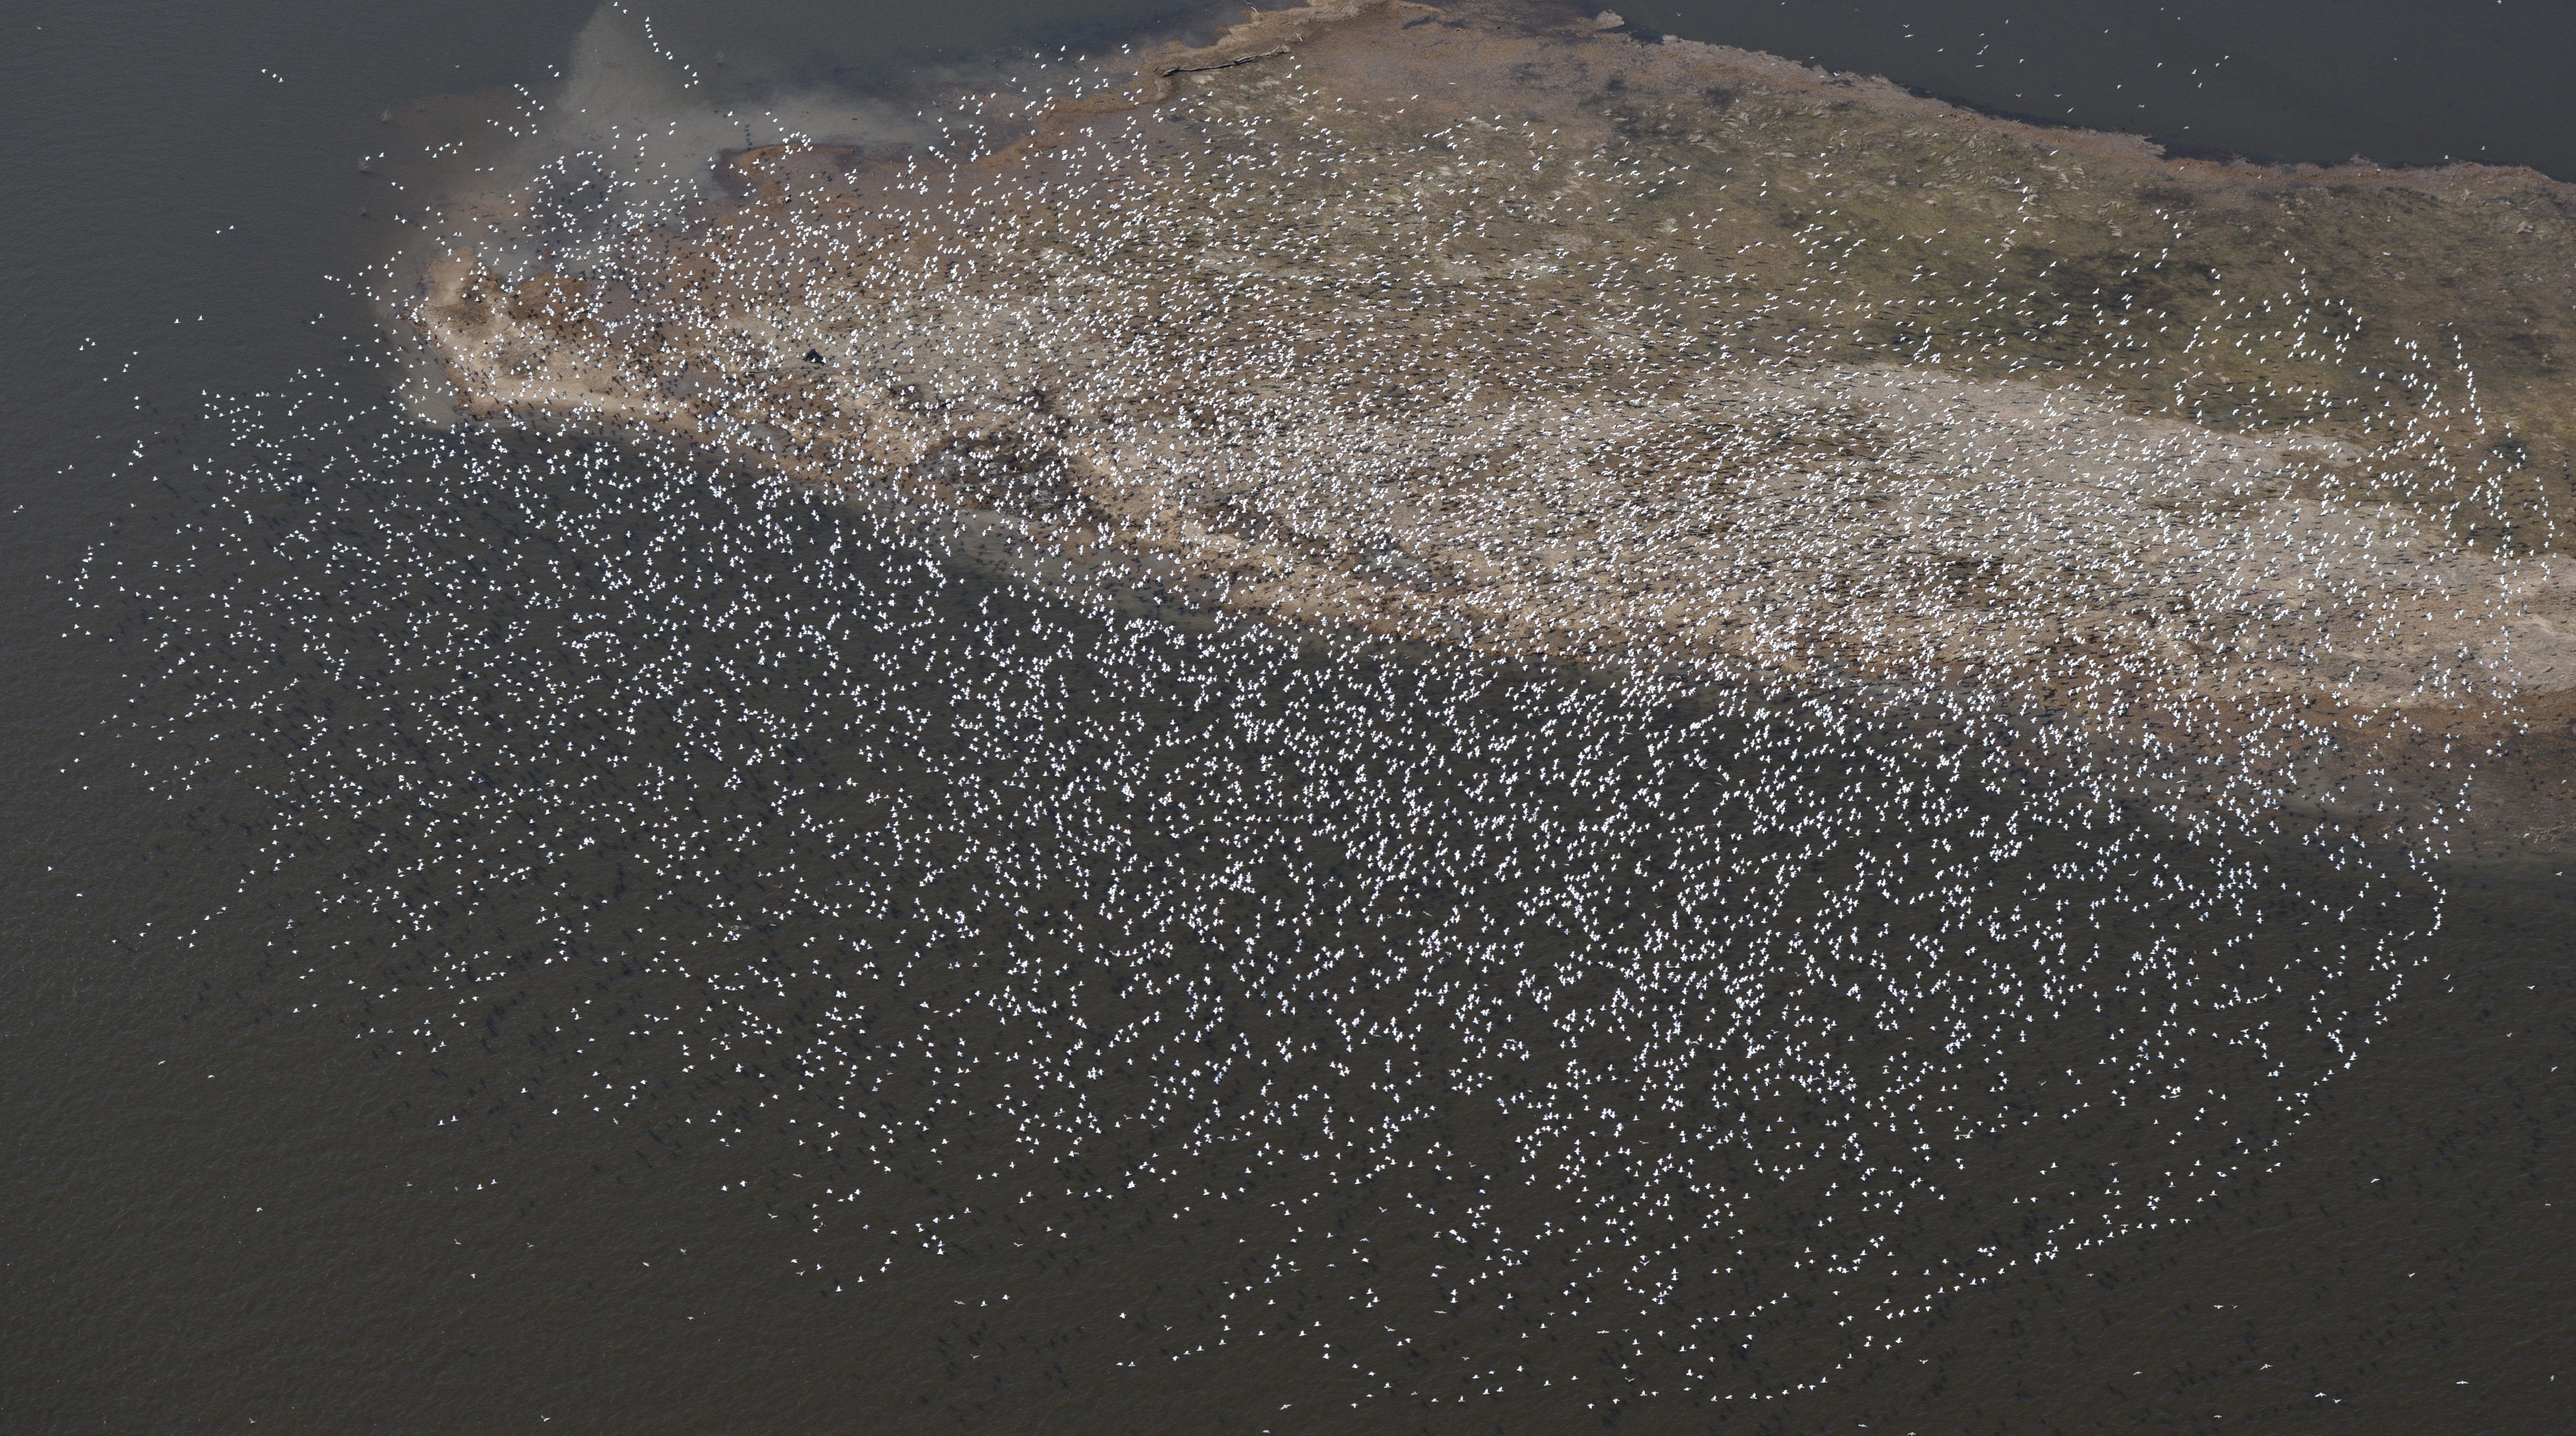
\includegraphics[width=80mm, height=50mm]{Figuras/GSGO_014_C_ES_ESTA.jpg}\par
    \caption{Photo of a flock of birds. The total number of birds in the photo is $N=13744$. (Photo obtained from: \href{https://datadryad.org/stash/dataset/doi:10.5061/dryad.98sf7m0hx}{DRYAD open data repository})}
    \label{fig:Foto_Pajaros}
  \end{subfigure}
  
  \caption{Photos from which the data that we analyze is obtained. The left photo is analyzed in the subsection 'Counting people' and the right photo is analyzed in the subsection 'Counting birds'.}
  \label{fig:Fotos}
  \end{center}
\end{figure}
%%%%%%%%%%%%%%%%%%%%%%%%%%%%%%%%%%%%%%%%%%%%%%%%%%%%%%%%%%%%%%%%%%%%%%%%%%%%%%%%%%%%%%%
\begin{figure}[h!]
  \begin{center}
  \begin{subfigure}[h!]{80mm}
    \includegraphics[width=80mm, height=50mm]{Figuras/PuntosPersonas.png}\par
    \caption{Points representing the group of people from Figure \ref{fig:Foto_Personas}. (Data used by \cite{personas})}
    \label{fig:Foto1}
  \end{subfigure}
  \hfill
  \begin{subfigure}[h!]{80mm}
    \includegraphics[width=80mm, height=50mm]{Figuras/PuntosPajaros.png}\par
    \caption{Points representing the flock of birds from Figure \ref{fig:Foto_Pajaros}. (Data obtained from: \href{https://datadryad.org/stash/dataset/doi:10.5061/dryad.98sf7m0hx}{DRYAD open data repository})}
    \label{fig:Foto2}
  \end{subfigure}
  
  \caption{Data points obtained from Figures \ref{fig:Foto_Personas} and \ref{fig:Foto_Pajaros}. The left image is analyzed in the subsection 'Counting people' and the right image is analyzed in the subsection 'Counting birds'.}
  \label{fig:Fotos_Puntos}
  \end{center}
\end{figure}


\subsection{Counting people}
%Resultados conteo (Histograma?????)
First, we will discuss the results obtained for the image in Figure \ref{fig:Foto_Personas}, which can be seen in Figure \ref{fig:NumberPeople}. Said image has a total amount of $N=4633$ people, whereas the mean estimated number of people using a test system of quadrats with $t=40$ and $T=120$ was $\widehat{N}\sim 4400$ considering every method and every set of points used.\\

%IMAGEN

If we now take a look at the different coefficient errors obtained, which can be seen in Figure \ref{fig:CountCoef}, they are all quite small with around $\sim 4$\% coefficient of error.\\ %Since the estimator that we are using is known to work well and (as we will see later comparing our results to other works) these results don't seem to give a sufficiently good estimator, the code that we are using for the test system of quadrats may not be implemented correctly.\\


%Histogramas coeficiente de error
Taking a better look at the histograms from Figure \ref{fig:CountCoef}, it looks like the CBC and Hinrichs methods have lower coefficient of error values when used with the $(x,y)$ process (with a few exceptions). Also, these values don't seem to vary that much when changing the number of optimal points considered. The method with the lowest coefficient of error value in this case is CBC $(x,y)$, however the Hinrichs $(x,y)$ method gets a similar value with less points considered (more efficiency).\\


%IMAGEN





\subsection{Counting birds}
%Resultados conteo (Histograma?????)
Now we will discuss the results obtained for the image in Figure \ref{fig:Foto_Pajaros}, which can be seen in Figure \ref{fig:NumberPajaros}. Said image has a total amount of $N=13744$ birds, whereas the mean estimated number of birds using a test system of quadrats with $t=44$ and $T=440$ was $\widehat{N}\sim 12700$ considering every method and every set of points used.\\

%IMAGEN

If we now take a look at the different coefficient errors shown in Figure \ref{fig:PajarosCoef}, they are all somewhat small with around $\sim 7$\% coefficient of error. However, \cite{conteo.pdf} obtained results for the same image, with the same parameters $(t,T)$ but only for $\omega = 60$º, giving a mean estimator $\widehat{N}=13700$ and a $0.3$\% mean coefficient error.\\ %Since their results are more satisfactory, our results don't seem to give a sufficiently good estimator even though the coefficient of error is small, which seems to indicate that the code is not correctly implemented.\\


%Histogramas coeficiente de error
Taking a better look at the histograms from Figure \ref{fig:PajarosCoef}, it looks like this time only the CBC method has lower coefficient of error values when used with the $(x,y)$ process for the majority of sets of points. Now the process $(x,\omega)$ has better results (lower coefficient of error values) for more sets of points when used with the Hinrichs method. Once again these values don't seem to vary that much when changing the number of optimal points considered. In regards to the best method, CBC has reached with two sets of points the lowest coefficient of error value with both processes ($(x,y)$ and $(x,\omega)$).\\


%IMAGEN






































\section{Buffon and Buffon-Steinhaus test systems}
In this subsection we will discuss the results obtained for the estimated curve length $\widehat{B}$ of different curves. Since the Buffon-Steinhaus test system is the union of two perpendicular Buffon test systems, we will explain the procedure used to count the intersections needed for equation \eqref{Buffon} by means of the Buffon test system. The same procedure applies for the Buffon-Steinhaus test system separately for each set of parallel lines that create the square grid.\\

The most important part of the procedure is the creation of the Buffon test system, namely the set of parallel lines that is "superimposed onto the curve". Now, in order to count the intersections we don't need to \textit{create} the test system, but rather \textit{check} if the points that conform the curve go past certain limits (meaning that we don't really superimpose the test system, but superimpose an imaginary test system instead). That being said, lets imagine that we want to create a test system of vertical lines separated a distance $T$ apart. So as to change the position and orientation of the whole test system, we attach an AV $(\widehat{x},\omega)$ to an AP $\widehat{x}=(x_1,x_2) \in \mathbb{R}^2$ of the test system. That way, the whole system moves depending on $\widehat{x}$ and rotates an angle $\omega \in [0,2\pi)$ with respect to the horizontal axis.\\


In order to obtain the number of intersections with the test system, the first step was to rotate the curve (which is equivalent to rotating the test system) an angle $\omega \in [0,\pi)$. We don't need to consider the full interval $[0,2\pi)$ since the same results are obtained in both cases due to the symmetry of the test system. The second step is to identify the AP of the test system, which for simplicity reasons was chosen to be the point $\widehat{x}=(m_x,m_y)$ with $m_x$ the lowest value of the first coordinate from all points conforming the curve and $m_y$ the lowest value of the second coordinate from all points conforming the curve. That way, for the purpose of maintaining randomness, a random value $r=(r_1,0) \text{ (mod T) } \in \mathbb{R}^2$ was added to $\widehat{x}$ (there is no need to consider a random value for the second coordinate since the vertical lines are infinite). Finally, to count the number of intersections between the curve and the test system, we checked whether two consecutive points conforming the curve happen to have the first coordinate lower and greater (or vice versa) than that of a specific line from the test system, respectively. If that is the case for some line, then an intersection is counted, otherwise no intersection is counted. Furthermore, this process was vectorized so that several values of $r$ and $\omega$ can be introduced respectively as \textit{arrays}, making the code more efficient.\\


%Procedimiento de Hinrichs
Lastly, we will explain how we implemented the optimal point sets for QMC integration in the code for this subsection. Similarly to last subsection, each test system created for the code has an AP $\widehat{x}$ with AV $(\widehat{x},\omega)\equiv(x_1,x_2,\omega)\equiv(x,y,\omega)$. Also, considering equation \eqref{QMC}, we have
\begin{equation*}
    \int_{\mathbb{R}^2} I(Y\cap \Lambda_{\textbf{x},\omega}) \,\mathrm{d}\textbf{x} \approx  \frac{1}{N} \sum_{n=0}^{N-1} I(Y\cap \Lambda_{\textbf{x}_n,\omega}),
\end{equation*}
where $\Lambda_{\textbf{x},\omega}$ is the Buffon test system and $\textbf{x}_n$, $n=0...,N-1$ are the optimal points for QMC integration. As a result, what we will do is calculate the number of intersections between the curve and the test system when the AP $\widehat{x}=(x,y)$ is located in each of the \textit{Hinrichs' optimal points} for bivariate periodic functions (namely the optimal points for QMC integration obtained in \cite{Hinrichs.pdf}, see Figure \ref{fig:Hinrichs} in the appendix). After that, those numbers calculated for each test system will be added and divided by the total number of Hinrichs' optimal points used, $N$. In consequence, this should give us the value $\mathbb{E}[I(Y\cap \Lambda_{\textbf{x},\omega})]$ with minimum worst case error. From now on, we will refer to this method as \textit{Hinrichs $(x,y)$}.\\

%Comentar el caso (x,w)
Again, we have also tried a different approach to this method. Apart from using the Hinrichs' optimal points in the AP $\widehat{x}=(x,y)$, we have also computed results where the first coordinate $x$ and the angle $\omega$ are modified by the optimal points for each system (see explanation in the latter subsection). From now on, we will refer to this method as \textit{Hinrichs $(x,\omega)$}. \\

\textbf{Notes:} 
\begin{itemize}
    \item In this subsection, we have also escalated the Hinrichs' optimal points depending on the method used.
    \item For the Buffon-Steinhaus test system we only have to use two perpendicular Buffon test systems and carry on the same procedure for each one of them.
\end{itemize}

\vspace{2mm}
We will now resume the computed results acquired for the estimated curve length $\widehat{B}$ of different curves and show how these methods' variances behave (via the squared coefficient of error (see equation \eqref{squaredCE})) compared to the other methods that have been presented in the last subsection. Again, these methods have also been tested for both the $(x,y)$ process and the $(x,\omega)$ process.\\

\textbf{Notes:} 
\begin{itemize}
    \item The results we show in this subsection have been obtained averaging the estimators computed for every possible translation and rotation.
    \item The results obtained for the original method have been computed but were not included in the Figures so as to get a better visualization of the other results. For the record, the estimators obtained with the original method are similar to those obtained with the other methods, but the error variance is much bigger.
\end{itemize}
\vspace{2mm}

%RESULTADOS
%Fotos
The curves whose length we tried to estimate can be seen in Figures \ref{fig:Pausinger} and \ref{fig:Curvas_ADN}.\\

\begin{figure}[h!]
  \begin{center}
    \includegraphics[width=80mm, height=50mm]{Figuras/CurvaBuffon.png}\par
    \caption{Image of a special symmetric curve obtained using the equation $ \gamma_{\textbf{a}}(t) = \sum_{j=0}^{m} \exp{2\pi i \textbf{a} t} $ from \cite{Pausinger.pdf} with $\textbf{a}=(1,3,4,11)$ ($m=4$). This curve is analyzed in the subsection 'Estimating length of Pausinger's curves'.}
    \label{fig:Pausinger}
  \end{center}
\end{figure}
%%%%%%%%%%%%%%%%%%%%%%%%%%%%%%%%%%%%%%%%%%%%%%%%%%%%%%%%%%%%%%%%%%%%%%%%%%%%%%%%%%%%%%%
\begin{figure}[h!]
  \begin{center}
  \begin{subfigure}[h!]{80mm}
    \includegraphics[width=80mm, height=50mm]{Figuras/Curva5.png}\par
    \caption{DNA molecule referred to as \textit{curve 5}.}
    \label{fig:Curva5}
  \end{subfigure}
  \hfill
  \begin{subfigure}[h!]{80mm}
    \includegraphics[width=80mm, height=50mm]{Figuras/Curva6.png}\par
    \caption{DNA molecule referred to as \textit{curve 6}.}
    \label{fig:Curva6}
  \end{subfigure}
  
  \caption{DNA molecules from \cite{adn.pdf} whose curve length is estimated. The left molecule is analyzed in the subsection 'Curve 5' and the right molecule is analyzed in the subsection 'Curve 6'.}
  \label{fig:Curvas_ADN}
  \end{center}
\end{figure}



\section{Estimating length of Pausinger's curves}
%Resultados longitud (Histograma?????)
First, we will discuss the results obtained for the image in Figure \ref{fig:Pausinger}, which can be seen in Figures \ref{fig:BuffonLength} and \ref{fig:Buffon-SteinhausLength}. The curve from that image has a total length in $\mathbb{R}^2$ $B=72.86$, accordingly, the mean estimated curve length obtained using the Buffon and Buffon-Steinhaus test systems with $T=1$ is $\widehat{B} \sim 72.87$ considering every method and every set of points used.\\

%IMAGEN
%IMAGEN


Looking at the different coefficient errors shown in Figures \ref{fig:BuffonCoef} and \ref{fig:Buffon-SteinhausCoef} they are all very small, with the biggest one being around $\sim 0.06$\% and the lowest one being around $\sim 0.001$\%. The estimator used is known to work well and these results seem really good with low error.\\


%Histogramas coeficiente de error
Taking a better look at the histograms from Figures \ref{fig:BuffonCoef} and \ref{fig:Buffon-SteinhausCoef}, it looks like the $(x,y)$ process (which in Buffon's test system it's called $(x)$ because changing the component $y$ doesn't modify the test system) is better (meaning that if gives a lower coefficient of error value) for all methods with the Buffon test system for all sets of points, however, with the Buffon-Steinhaus test system the process $(x,y)$ is only better for all point sets with the Fictional and Hinrichs methods. The CBC method with a Buffon-Steinhaus test system is mostly better when used with the process $(x,y)$, however, there are some exceptions. About the values that the coefficient of error takes, there seems to be a relation between these values and the number of optimal points considered for all methods with the $(x,y)$ process except the CBC method with a Buffon-Steinhaus test system, which could mean that more points equals more precision. It is worth mentioning that the fictional $(x,y)$, fictional $(x,\omega)$ and Hinrichs $(x,y)$ methods give the same values when used with the Buffon and Buffon-Steinhaus test systems for any set of points considered. This is because the symmetry of those test systems makes it so fictional $(x,y)$ and fictional $(x,\omega)$ are equal to one another and the process considered to obtain the AP of the test systems gives equivalent sets of points for the fictional and Hinrichs methods (modulo the test system's symmetry). All the methods have reached the lowest coefficient of error value with the $(x,y)$ process using both the Buffon and the Buffon-Steinhaus test systems.\\


%IMAGEN
%IMAGEN







\section{Estimating length of DNA molecules}
%Resultados conteo (Histograma?????)
%%%%%%%%%%%%%%%%%%%%%%%%%%%%%%%%%%%%%%CURVA 5
Now we will discuss the results obtained for the images in Figure \ref{fig:Curvas_ADN}. 

\subsection{Curve 5}
We will start talking about the DNA molecule in Figure \ref{fig:Curva5}, which we will refer to as \textit{Curve 5} because of how it's numerated by \cite{adn.pdf}. The results for curve 5 can be seen in Figures \ref{fig:C5BuffonLength07} and \ref{fig:C5Buffon-SteinhausLength07}. Curve 5 has a total length in $\mathbb{R}^2$ $B=12.78$, accordingly, the mean estimated curve length obtained using the Buffon and Buffon-Steinhaus test systems with $T=0.7$ are $\widehat{B} \sim 12.76$ and $\widehat{B} \sim 12.80$ respectively considering every method and every set of points used.\\


%IMAGEN
%IMAGEN


Taking a look at the different coefficient errors shown in Figures \ref{fig:C5BuffonCoef07} and \ref{fig:C5Buffon-SteinhausCoef07} they are all very small, with the biggest one being around $\sim 2$\% and the lowest one being around $\sim 0.02$\%, making the results seem really good with low error. \cite{adn.pdf} analyzed the same curve and obtained a curve length $B=393$ nm and estimated curve length $\widehat{B}=333$ nm with a coefficient error $11.6$\% using a Buffon-Steinhaus test system (square grid) with $T=25$ nm. On their work they take $T=25$ nm so as to get an intersection expectation $\mathbb{E}[I] \sim 20$ intersections. In our case $T=0.7$ was chosen, leading to $\mathbb{E}[I] \sim 10$ intersections (per optimal point) for the Buffon test system and $\mathbb{E}[I] \sim 20$ intersections (per optimal point) with the Buffon-Steinhaus test system. It seems like we are getting better results in this case for curve length estimation.\\



%Histogramas coeficiente de error
Contrary to what we saw in the counting results, taking a better look at the histograms from Figures \ref{fig:C5BuffonCoef07} and \ref{fig:C5Buffon-SteinhausCoef07} we see that the $(x)$ process for the Buffon test system is worse in this case for all methods but the fictional (for any set of points considered). However, just like last time, coefficient of error values tend to lower when more optimal points are considered using the CBC and Hinrichs methods, but this time with the $(x,\omega)$ process. About the histograms for the Buffon-Steinhaus test system, the coefficient of error values seem random (no relation between number of points and coefficient of error value) and there doesn't seem to be a better process between the $(x,y)$ and the $(x,\omega)$ in general. For the majority of sets of points the $(x,y)$ process is better with the Hinrichs method (with exceptions), but with the CBC method the $(x,\omega)$ process looks better for the vast majority of sets of points (with few exceptions). Also, we can see again that the fictional $(x,y)$, fictional $(x,\omega)$ and Hinrichs $(x,y)$ methods give the same values when used with the Buffon and Buffon-Steinhaus test systems for any set of points considered. The method with the lowest coefficient of error value in this case is CBC with the $(x,\omega)$ process for both the Buffon and the Buffon-Steinhaus test systems.\\



%IMAGEN
%IMAGEN






%%%%%%%%%%%%%%%%%%%%%%%%%%%%%%%%%%CURVA 6
\subsection{Curve 6}
Lastly, we will discuss the results obtained for the DNA molecule in Figure \ref{fig:Curva6}, which we will refer to as \textit{Curve 6} because of how it's numerated by \cite{adn.pdf}. The results for curve 6 can be seen in Figures \ref{fig:C6BuffonLength07} and \ref{fig:C6Buffon-SteinhausLength07}. Curve 6 has a total length in $\mathbb{R}^2$ $B=15.16$, accordingly, the mean estimated curve length obtained using the Buffon and Buffon-Steinhaus test systems with $T=0.7$ are $\widehat{B} \sim 15.24$ and $\widehat{B} \sim 15.19$ respectively considering every method and every set of points used.\\

%IMAGEN
%IMAGEN


Taking a look at the different coefficient errors shown in Figures \ref{fig:C6BuffonCoef07} and \ref{fig:C6Buffon-SteinhausCoef07} they are all quite small, with the biggest one being around $\sim 7$\% and the lowest one being around $\sim 0.009$\%, making the results seem really good with low error. \cite{adn.pdf} analyzed the same curve and obtained a curve length $B=392$ nm and estimated curve length $\widehat{B}=351$ nm with a coefficient error $11.2$\% using a Buffon-Steinhaus test system (square grid) with $T=25$ nm. This time $T=0.7$ led to $\mathbb{E}[I] \sim 14$ intersections (per optimal point) for the Buffon test system and $\mathbb{E}[I] \sim 28$ intersections (per optimal point) with the Buffon-Steinhaus test system. Again, it seems like we get better results for curve length estimation.\\



%Histogramas coeficiente de error
Once again, contrary to what we saw in the first length estimation results, taking a better look at the histograms from Figures \ref{fig:C5BuffonCoef07} and \ref{fig:C5Buffon-SteinhausCoef07} we see that the $(x)$ process for the Buffon test system is worse for all methods but the fictional (for any set of points considered). Also, similarly to the results for curve 5, coefficient of error values tend to slightly lower when more optimal points are considered using the CBC and Hinrichs methods with the $(x,\omega)$ process. However, about the histograms for the Buffon-Steinhaus test system, even though the coefficient of error values still seem random (no relation between number of points and coefficient of error value) it's clear that the $(x,\omega)$ process is better for all methods but the fictional. Also, we can see again that the fictional $(x,y)$, fictional $(x,\omega)$ and Hinrichs $(x,y)$ methods give the same values when used with the Buffon and Buffon-Steinhaus test systems for any set of points considered. Once more, the method with the lowest coefficient of error value is CBC with the $(x,\omega)$ process for both the Buffon and the Buffon-Steinhaus test systems.\\


%IMAGEN
%IMAGEN




Finally we will mention a few other results that were obtained during the development of the code for the Buffon-Steinhaus test system.  We checked that the Hinrichs $(x,y)$ method provides an estimator with the same variance as the original method when considering the same number of evaluations. This means that, for example, if one chooses a Buffon-Steinhaus test system with $T=0.1$ and uses the original method then the estimator's variance will be similar to the one obtained for a Buffon-Steinhaus test system with $T=1$ used with the Hinrichs $(x,y)$ method considering $N=10$ optimal points. On the other hand, the Hinrichs $(x,\omega)$ and CBC methods give worse results in this case. We also checked that the estimator's variance decreases when the value of the parameter $T$ decreases, this makes sense because doing so we are lowering the chances for test system to intersect the curve in places where the number of intersections changes significantly. Moreover, we can say that, from all the experiments (for all test systems used in this work) that have been carried out, the computing time didn't seem to exceed the five minute mark. Considering that \cite{conteo.pdf} and \cite{adn.pdf} had computing times of around five minutes or more with less function evaluations, this indicates that our code is very efficient.\\










%EXTRAS

%Mixing the results from curves 5 and 6, one might think that using Hinrichs $(x,\omega)$ might be better than using Hinrichs $(x,y)$ depending on whether the curve analized is isotropic or anisotropic (see \cite{adn.pdf}).\\ No parece ser eso????
%Pausingers curve
In conclusion, at least one of the CBC and Hinrichs methods seems to give the lowest coefficient of error values when used with the $(x,\omega)$ and $(x,y)$ processes respectively. However, it is possible that one method is better than the other depending on the isotropy, anisotropy or symmetry that the analyzed object has (in this case the curve or the group of points from the photo). It is also possible that changing the value of the parameter $\gamma$ mentioned in \cite{Hinrichs.pdf} provides better results for the Hinrichs method in every experiment. Nonetheless, the Hinrichs method seems to give low coefficient of error values at least for one of the processes $(x,y)$ or $(x,\omega)$, which makes it a and easy-to-implement estimation method for stereology.\\






